\documentclass[12pt]{article}
\usepackage[utf8]{inputenc}
\usepackage{amsmath}
\usepackage{multicol}
\usepackage{graphicx}
\usepackage{float}
\usepackage{dsfont}
\usepackage{textcomp}
\usepackage{amsfonts}
\usepackage{hyperref}
\usepackage{amsmath}
\usepackage{csquotes}
\usepackage[style=authoryear,backend=biber]{biblatex}
\addbibresource{mybib.bib}
\hypersetup{
    colorlinks,
    citecolor=black,
    filecolor=black,
    linkcolor=black,
    urlcolor=black
}
\usepackage{cleveref}
\usepackage{fancyhdr}
\setlength{\headheight}{14.5pt}
\renewcommand{\sectionmark}[1]{\markright{#1}{}}
\usepackage[T1]{fontenc}
\usepackage[colorinlistoftodos]{todonotes}
\usepackage[margin=2cm,a4paper]{geometry}
\newgeometry{left=2.0cm,right=2.0cm,top=2.5cm,bottom=2.5cm}
\usepackage{listings}
\setlength{\marginparwidth}{2cm}
\setlength{\parindent}{0pt}
\newcommand{\deriv}{\mathrm{d}}
\title{}
\pagestyle{fancy}
\fancyhf{}
\rhead{Section \thesection}
\lhead{Assignment 1: Data Mining in Virtual Observatories}
\lfoot{PH512: Data Analysis Techniques in Astronomy and Planetary Science}
\rfoot{Page \thepage}
\renewcommand{\headrulewidth}{1pt}
\renewcommand{\footrulewidth}{1pt}
\begin{document}
\begin{titlepage}
\newgeometry{left=1.0in,right=1.0in,top=0.8in,bottom=0.8in}
\newcommand{\HRule}{\rule{\linewidth}{0.5mm}}
\begin{centering} 

%---------------------------------------------------------------------------
%	TITLE SECTION
%---------------------------------------------------------------------------

\includegraphics[scale=0.7]{Images/Uni_of_Kent.png}\\[1cm]
\HRule \\[0.4cm]
\Huge{\bfseries{Data Mining in Virtual Observatories}}\\[0.1cm]
\textsc{\large Data Analysis Techniques in Astronomy and Planetary Science}\\[0.1cm]
\textsc{\large BSc(Hons) Astronomy, Space Science and Astrophysics}\\[0.1cm]
\HRule \\[0.5cm]
%---------------------------------------------------------------------------
\begin{minipage}{0.625\textwidth}
\begin{center} \large
{\large Author: Lukasz R Tomaszewski (lrgt2)} \\[0.2cm]
{\large Date: $15^{th}$ - $29^{th}$ January 2020}\\[0.2cm]
{\large PH512 Assignment 1} \\[0.2cm]
{\large Word Count: 1354} \\
\end{center}
\end{minipage}\\[1cm]
\end{centering} 
\begin{tableofcontents}
\end{tableofcontents}
\end{titlepage}
\newpage
%---------------------------------------------------------------------------
%	SECTION 1
%---------------------------------------------------------------------------
\section{'fits' datafiles, 'jpg' \& 'gif' formats}
\label{Section 1}

Astronomers across the globe use a NASA endorsed file format called ’fits’ (Flexible Image Transport System) as it defines a standard for all astronomers to adhere to so they can exchange files easily between new/old telescopes and or image software. A 'fits' file contains 3 main components: the header, image data and the tailer. The header is the name of the file written in ASCII characters that allows humans and computers to find and isolate the file, the image data is a log of binary data that is converted into a image when applied to certain software but when the image data is much smaller than another a tailer is added that adds extra bytes to the file to fill a standardized length, though rarely used (\cite{ImageProcessing}). \\

Whereas comparing 'jpg' (Joint Photograpic expert Group) and 'gif' (Graphics Interchange Format) where both are compressible but differ in file size and quality. The 'jpg' format offers a larger colour palette than the 'gif' format (\cite{Jpgvsgif1}), thus higher quality which is why its used for photographs but 'gif' stores multiple images and allows an animation to take place. As astronomers share images, compressing the large file size into a smaller file size allows for easier distribution but 'jpg' images loss image data with each compression and thus loses it image quality with each compression (\cite{Jpgvsgif2}), this has a negative effect on astronomer who require very detailed image quality. \\

%---------------------------------------------------------------------------
%	SECTION 2
%---------------------------------------------------------------------------
\section{Aladin analysis of the Messier 61 galaxy}
\label{Section 2}

By observing the spiral Messier 61 galaxy with the naked eye, these images were taken in March 1991 using the 48-inch (1.2-meter) Samuel Oschin Telescope, possessing a 72-inch (1.8-meter) f/2.5 mirror and used square photographic plates 14-inch (35.5-cm) in size, It would only be until 9 years later that four modern CCD cameras would replace them (\cite{Telescope}). \\

The angular resolution of the resourced images is embedded in its 'fits' header and have the values of $1.009^{\prime \prime}$ by $1.007^{\prime \prime}$ which allows the telescope to distinguish between small object i.e. better image quality. With the image scaling $891\times893$ pixels (roughly $14.98^{\prime}$$\times$$14.99^{\prime}$), at 16 bits per pixel with a pixel size of 15.03$\times$ 15.00 microns in the x,y plane. The FOV (field of view) is calculated by measuring the angular length of the target object and for the M61 galaxy is $4.22^{\prime}$ by $5.023^{\prime}$.\\

Calculating the pixel scale using; \\

\begin{equation}
Pixel \hspace{0.1cm} Scale[^{\prime \prime}] = \dfrac{206 * \hspace{0.1cm} (x,y) Pixel \hspace{0.1cm} size}{Focal \hspace{0.1cm} length} 
\end{equation}

\begin{equation}
    \begin{array}{l}
    X_{axis} = \dfrac{206 \times 15.03 microns}{1828.8mm} = 1.693^{\prime \prime} / Pixel \\ [0.5cm]
    Y_{axis} = \dfrac{206 \times 15.00 microns}{1828.8mm} = 1.689^{\prime \prime} / Pixel
    \end{array}
\end{equation}

\begin{multicols}{2}
\begin{figure}[H]
\centering
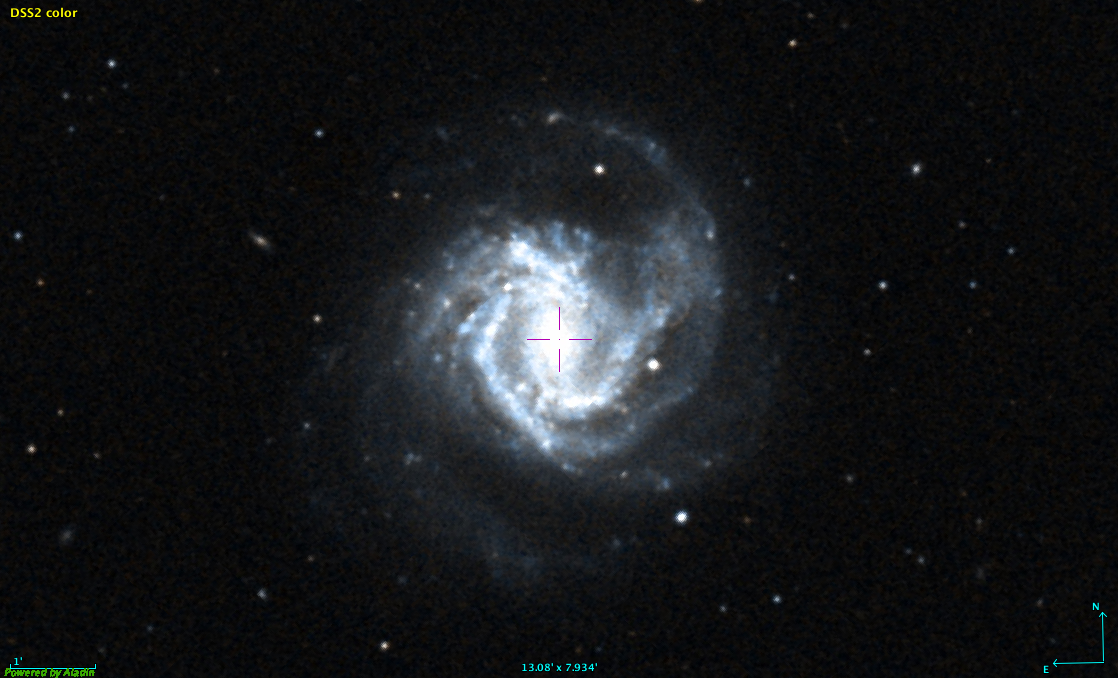
\includegraphics[scale=0.22]{Images/As_Images/M61.png}
\caption{Aladin image of the Messier 61 galaxy in the visible wavelength spectrum.}
\label{Aladin image of the Orion Nebula}
\end{figure}

\begin{figure}[H]
\centering
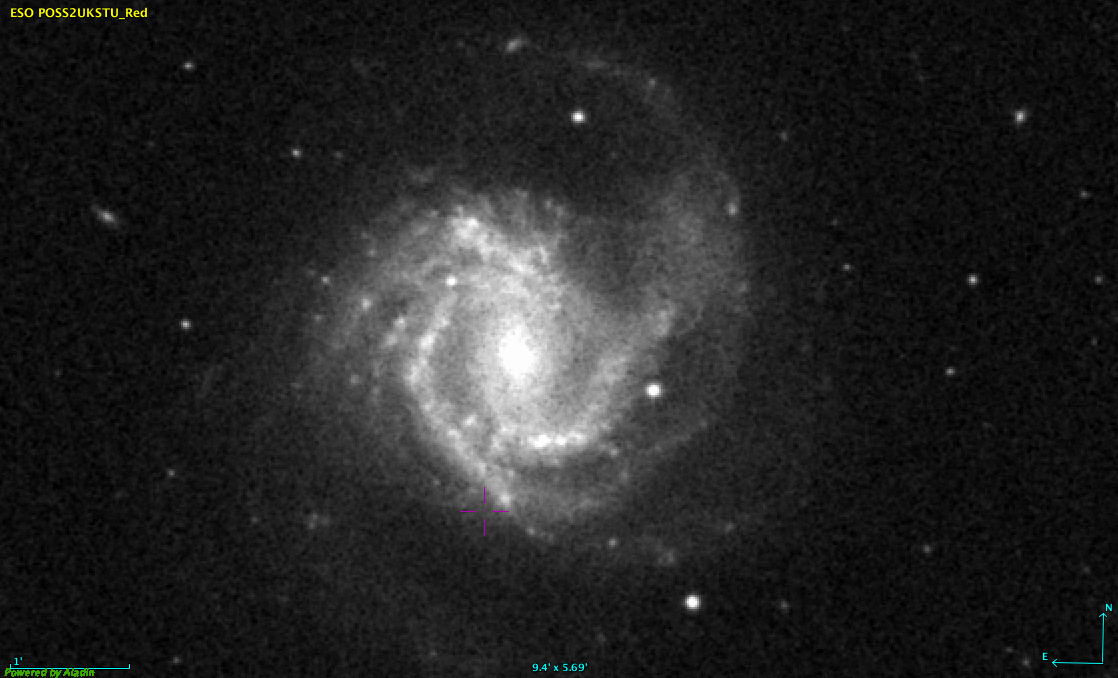
\includegraphics[scale=0.22]{Images/As_Images/M61Red.png}
\caption{Aladin image of the Messier 61 galaxy in the red 700nm wavelength spectrum.}
\label{Aladin Red image of the Orion Nebula}
\end{figure}
\end{multicols}
\vspace{0.2cm}

The Rayleighs criterion for the resolution image (minimum resolvable detail) is given by \cref{rayleighs} and the diameter of the Messier 61 galaxy can be calculated using trigonometry in spherical coordinates in \cref{S}. \\

\begin{equation}
\begin{array}{l}
    {\alpha}_{R-IR} = \dfrac{1.22 \hspace{0.1cm \lambda}}{D} \rightarrow \dfrac{1.22 \hspace{0.1cm * 700nm}}{1800mm} = 4.744{_{x10}}^{-10} \\ [0.5cm]
    {\alpha}_{R-Blue} = \dfrac{1.22 \hspace{0.1cm \lambda}}{D} \rightarrow \dfrac{1.22 \hspace{0.1cm * nm}}{1800mm} = 3.050{_{x10}}^{-10}
\end{array}
\label{rayleighs}
\end{equation}
\vspace{0.3cm}

\begin{equation}
S = r \hspace{0.1cm} \theta
\label{S}
\end{equation}
\vspace{0.2cm}

As \cref{S} is in spherical coordinates, $\theta$ is in radians, by using the distance tool, a value in arc minutes will be obtained where it can be converted into degrees and then radians, the value of r = 16.86 MPc (\cite{Distance}) and $\theta = 0.001746$ [Rads]. \\

\begin{equation}
S = {16.86}_{{x10}^6} \hspace{0.1cm} [Pc] \hspace{0.1cm} \times \hspace{0.1cm} 0.001746 \hspace{0.1cm}[Rads] = 29437.56 \hspace{0.1cm} [Pc]
\label{Diameter}
\end{equation}
\vspace{0.2cm}

The approximated diameter of the Messier 61 galaxy is 30660.139 [Pc] (\cite{Diameter}) where in \cref{Diameter} its deduced from the resourced images to be 29437.56 [Pc] which is 1222.579 [Pc] less, analysis concluded that an error in measuring the correct angle length using the distance tool on the image. \\

Lastly depicted in \cref{Aladin profile image of the Messier 61 galaxy} is the light intensity of the Messier 61 galaxy from \cref{Aladin IR image of the Orion Nebula} produced a FWHM (Full Width Half Maximum) value of 99.9 Pix/$1.682^{\prime}$ with a pixel value of 12888. 

%---------------------------------------------------------------------------
%	SECTION 3
%---------------------------------------------------------------------------
\section{Further analysis of the Messier 61 galaxy}
\label{Section 3}

All of the Aladin images are taken in gray scale where there is no colour, the 'RGB' tool allows the three wavelengths; red, blue and infrared, these are all combined to produce a true colour image that can be manipulated by changing the colour levels and contrast. Analysing \cref{RGB Aladin image of the Messier 61 galaxy} where the green wavelength is more prominent (even though no image was taken in the green wavelength spectrum) as the red and blue colour wavelengths are decreased whereas is \cref{RGB2 Aladin image of the Messier 61 galaxy} the blue wavelength is more prominent. This tool allows for a further understanding into the target objects prominent wavelength i.e. in this case its the blue wavelength. \\

\begin{multicols}{2}
\begin{figure}[H]
\centering
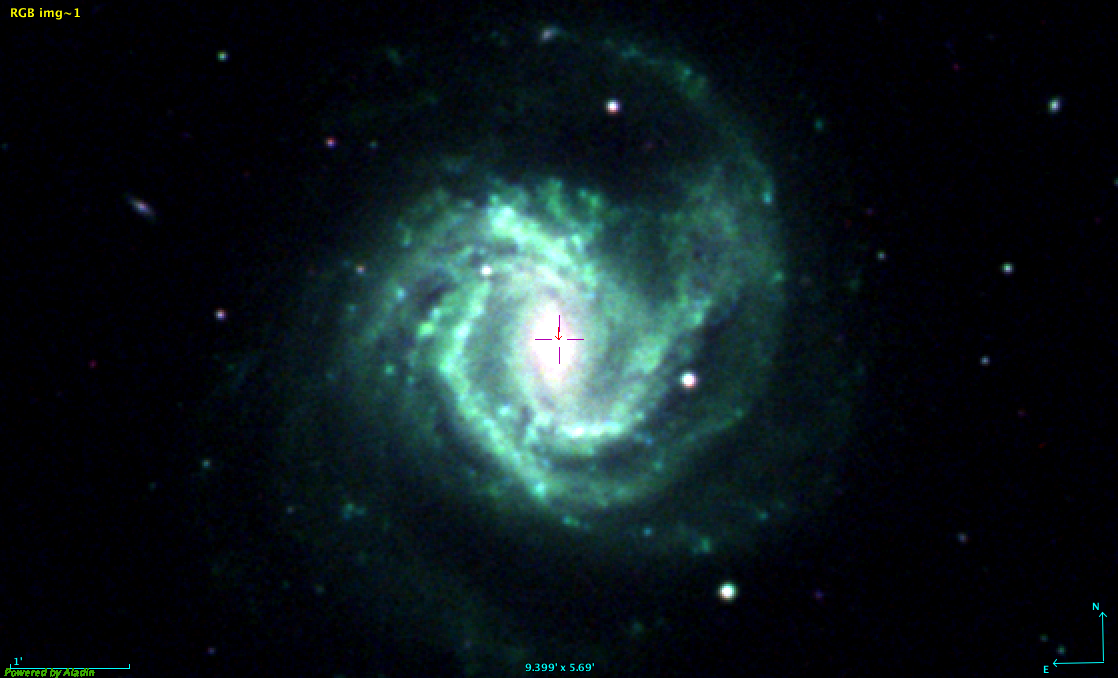
\includegraphics[scale=0.22]{Images/As_Images/M61RGB.png}
\caption{Aladin false-colour RGB image of the Messier 61 galaxy.}
\label{RGB Aladin image of the Messier 61 galaxy}
\end{figure}

\begin{figure}[H]
\centering
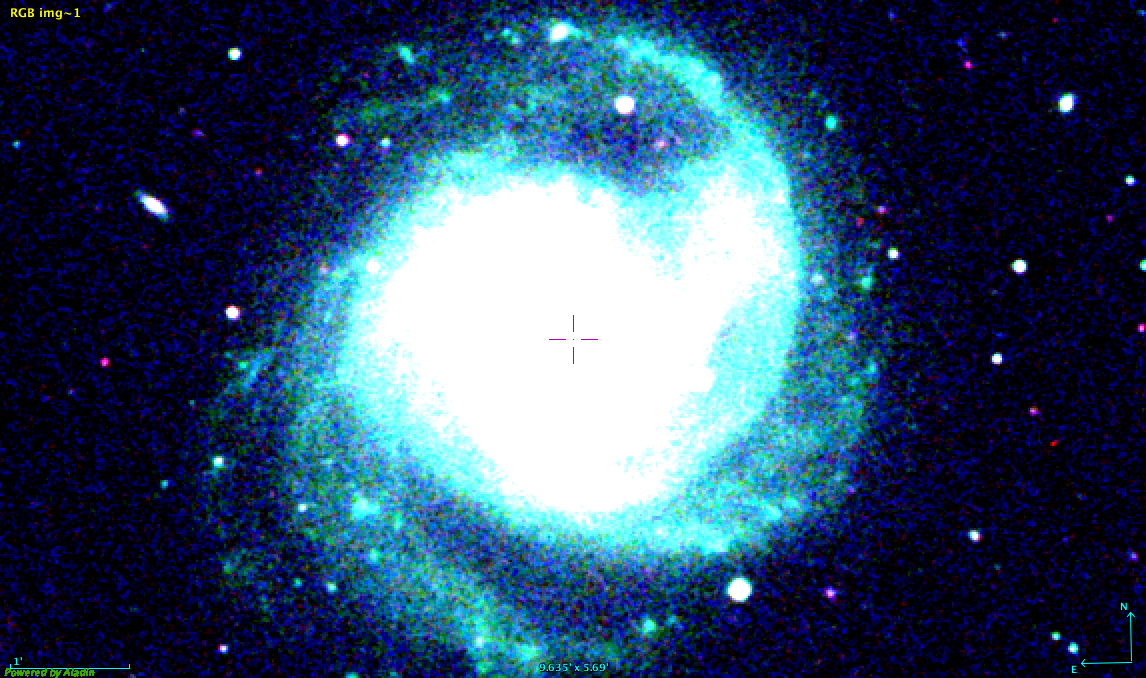
\includegraphics[scale=0.22]{Images/As_Images/M61RGB2.png}
\caption{Aladin false-colour RGB image of the Messier 61 galaxy.}
\label{RGB2 Aladin image of the Messier 61 galaxy}
\end{figure}
\end{multicols}

\begin{multicols}{2}
\begin{figure}[H]
\centering
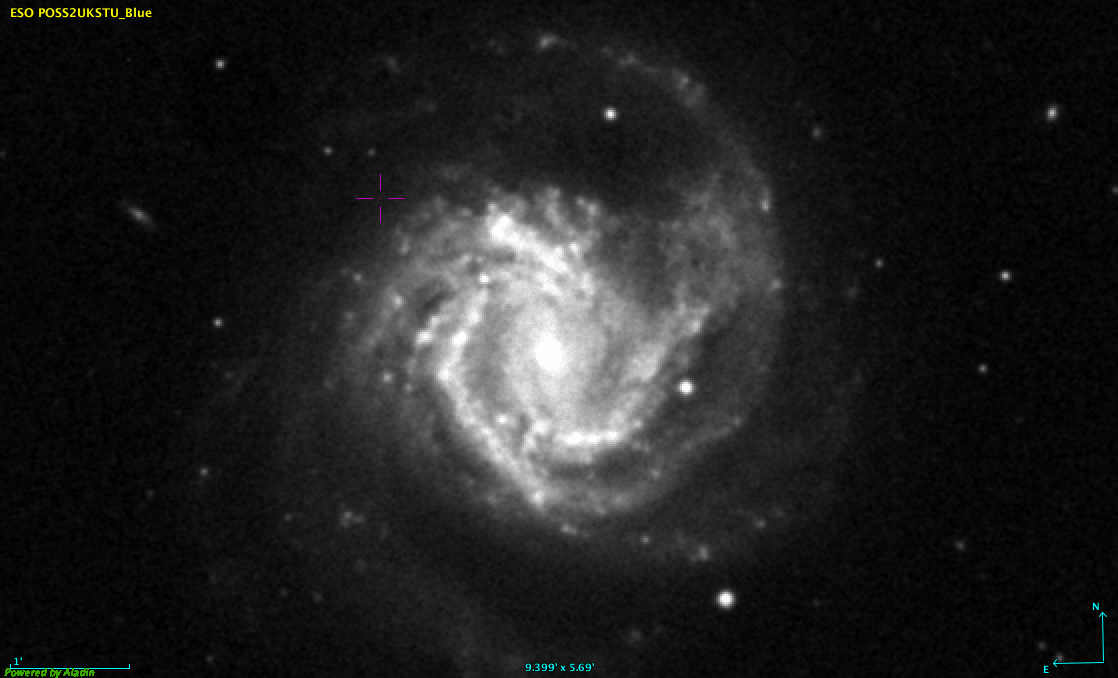
\includegraphics[scale=0.22]{Images/As_Images/M61Blue.png}
\caption{Aladin image of the Messier 61 galaxy in the blue 450nm wavelength spectrum.}
\label{Aladin Blue image of the Orion Nebula}
\end{figure}

\begin{figure}[H]
\centering
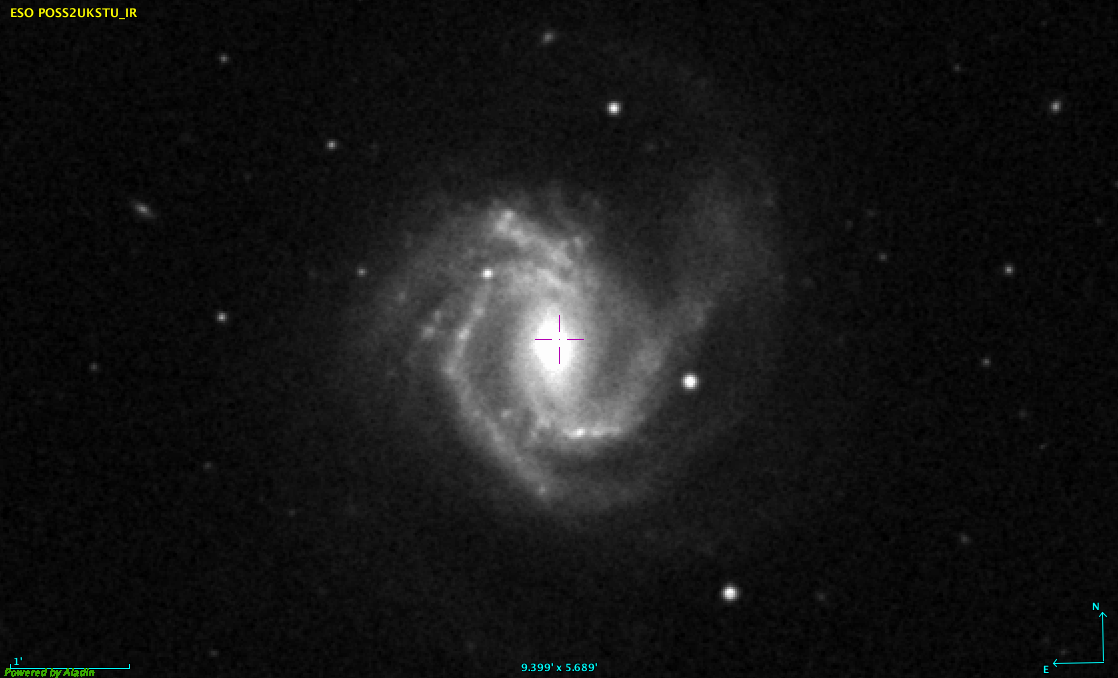
\includegraphics[scale=0.22]{Images/As_Images/M61IR.png}
\caption{Aladin image of the Messier 61 galaxy in the infrared 700nm-1mm wavelength spectrum.}
\label{Aladin IR image of the Orion Nebula}
\end{figure}
\end{multicols}
\vspace{0.2cm}

Furthermore comparing the blue, red and infrared wavelengths depicted in \cref{Aladin Blue image of the Orion Nebula}, \cref{Aladin Red image of the Orion Nebula} and \cref{Aladin IR image of the Orion Nebula}, the Messier 61 galaxy is rich in colour through the visible light spectrum thus can be seen with the naked eye. The telescope captures images of its target object in a specific wavelength thus allowing astronomers to be able to analyse the astronomical objects electromagnetic radiation produced by each individual wavelength. 

The contour tool allows the image to isolate different intensities of light (isophotes), in one layer all of the light intensity (isophotes) is the same, the number of levels with respect to their targeted light intensity value both can be altered to allow deeper analysis of the galaxy. When looking at a segment or star system in the Messier 61 galaxy, the contour tool allows for further isolation of each of the isophote intensities as well as the option to manipulate the amount of levels generated with each desired intensity value. This feature allows astronomers to separate background light radiation for different systems with in the galaxy to which a light intensity profile can be made. 

\begin{multicols}{2}
\begin{figure}[H]
\centering
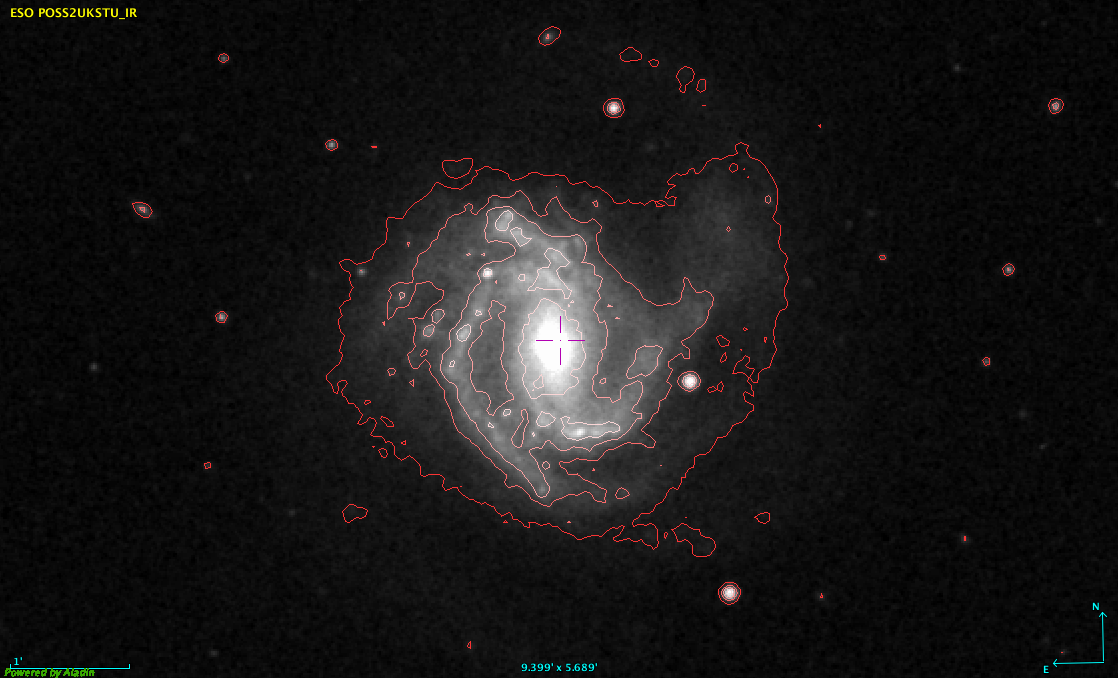
\includegraphics[scale=0.22]{Images/As_Images/M61IRContour.png}
\caption{Aladin contour image of the Messier 61 galaxy in the infrared wavelength spectrum.}
\label{Aladin IR Contour image of the Messier 61 galaxy}
\end{figure}

\begin{figure}[H]
\centering
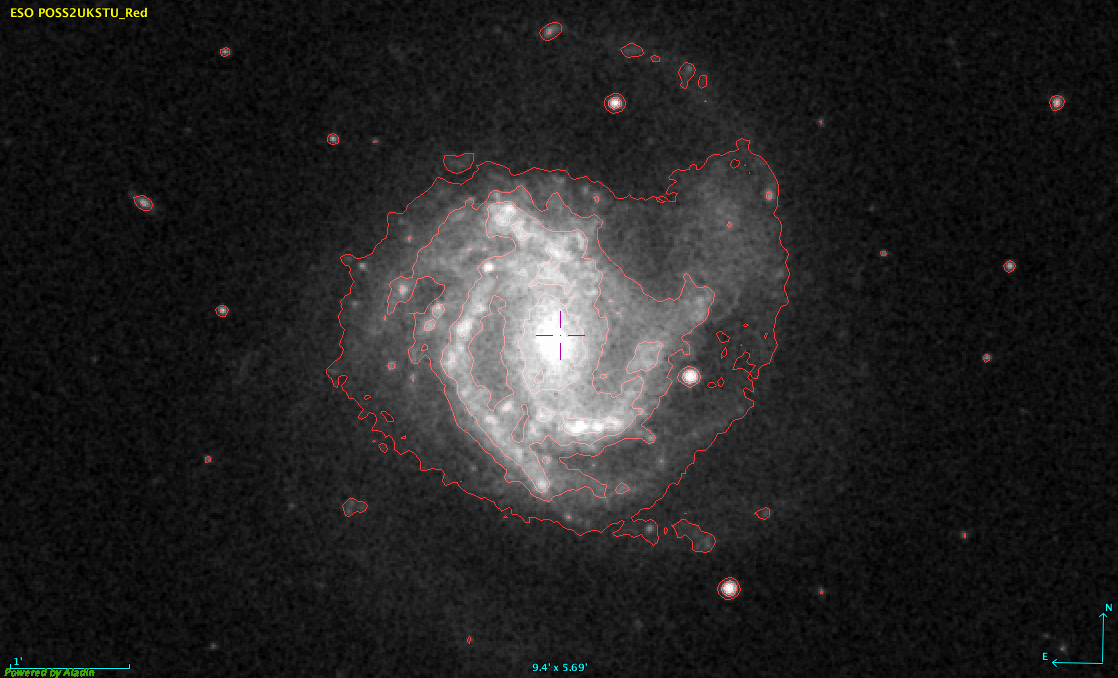
\includegraphics[scale=0.22]{Images/As_Images/M61RedContour.png}
\caption{Aladin contour image of the Messier 61 galaxy in the red wavelength spectrum.}
\label{Aladin Red Contour image of the Messier 61 galaxy}
\end{figure}
\end{multicols}

\begin{multicols}{2}
\begin{figure}[H]
\centering
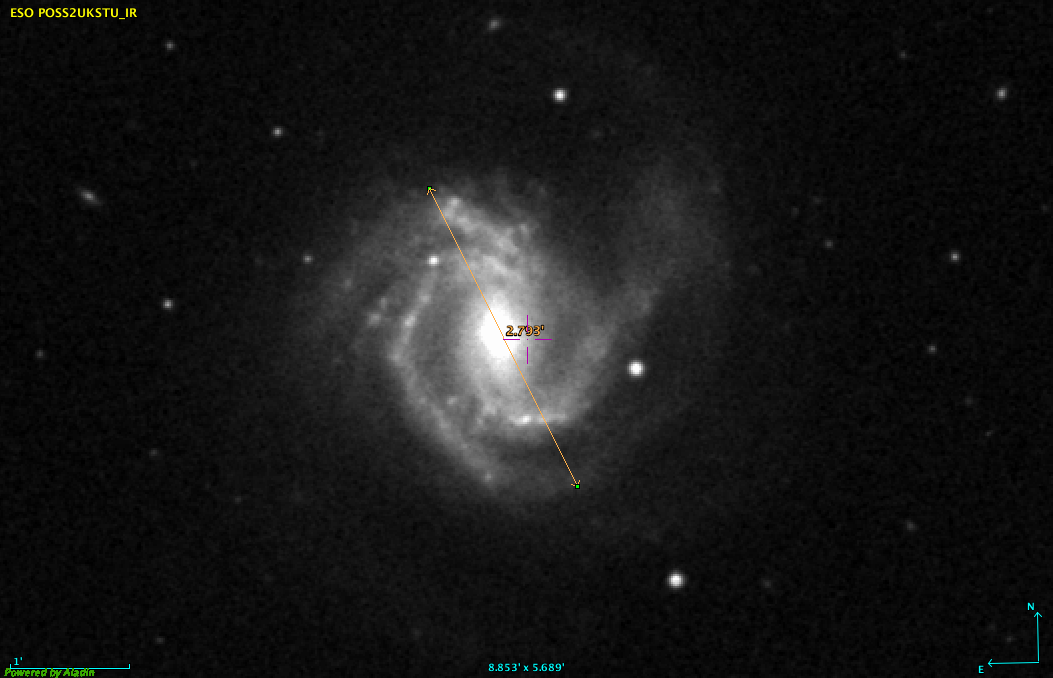
\includegraphics[scale=0.22]{Images/As_Images/M61Cut.png}
\caption{Cutting the Aladin image of the Messier 61 galaxy in the infrared wavelength spectrum.}
\label{Aladin IR Cut Profile image of the Messier 61 galaxy}
\end{figure}

\begin{figure}[H]
\centering
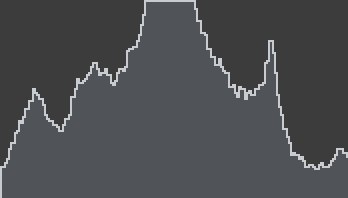
\includegraphics[scale=1.4]{Images/As_Images/M61Profile.png}
\caption{Aladin profile image of the Messier 61 galaxy in the infrared 700nm-1mm wavelength spectrum.}
\label{Aladin profile image of the Messier 61 galaxy}
\end{figure}
\end{multicols}
\vspace{0.2cm}

Utilizing the 'cut graph' tool in \cref{Aladin IR Cut Profile image of the Messier 61 galaxy}, a line measurement across the diameter is made through the centre of the galaxy in which a 'profile' is graphed in \cref{Aladin profile image of the Messier 61 galaxy} which shows the light intensity across the line measurement. Its peaks highlight an increase in luminosity (most likely astronomical objects appear here) and the troughs show low levels of luminosity, where its blank space but doesn't drop so sharply due to light reflection/ radiation off nearby stars. The luminosity of a star shows hot spots such as solar flares but for a galaxy the profile graph shows much more as the main features for astronomical objects are closely related to its luminosity and brightness.\\

\begin{figure}[H]
\centering
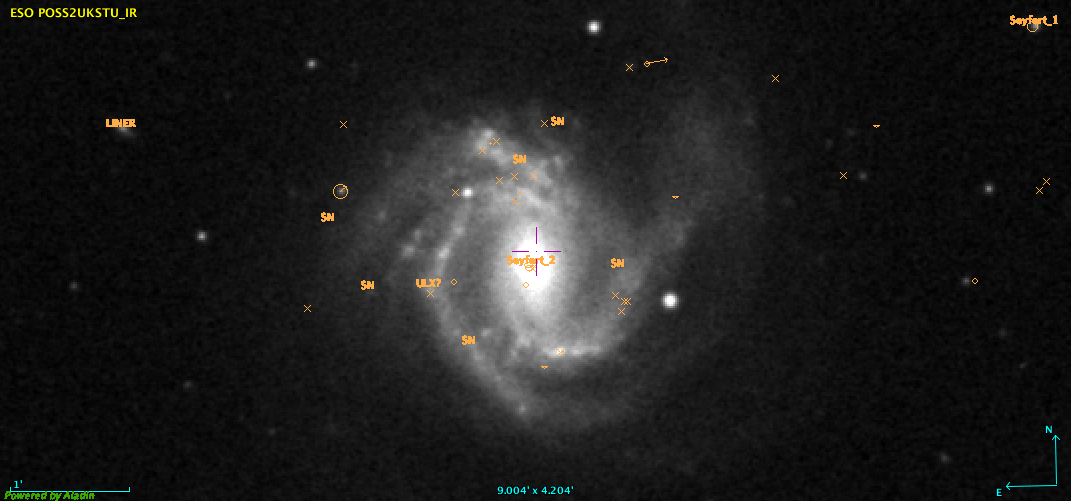
\includegraphics[scale=0.45]{Images/As_Images/M61Simbad.png}
\caption{Aladin Simbad image of the Messier 61 galaxy in the infrared wavelength spectrum.}
\label{Aladin Simbad image of the Messier 61 galaxy}
\end{figure}

All of these tools in the Aladin program can assist astronomers into isolating individual astronomical objects which are recorded and with the help of the 'fits' format, astronomers can study these objects. The 'Simbad' database features a map and lists all the recorded astronomical objects as seen in \cref{Aladin Simbad image of the Messier 61 galaxy}, from the naked eye most of these objects cannot be seen so the 'Simbad' database feature gives astronomers the ability to further analyse the astronomical object. 

%---------------------------------------------------------------------------
%	SECTION 4
%---------------------------------------------------------------------------
\section{Discussion of the Messier 61 galaxy}
\label{Section 4}

The Messier 61 galaxy is a barred spiral galaxy located in the Virgo cluster with a NGC 4303 core (\cite{Simbad}) where a vast amount of blue 450nm electromagnetic wavelength radiation is detected, this electromagnetic radiation forms an electromagnetic field off the light sources of each individual star and or astronomical object within the Messier 61 galaxy. As the blue wavelength spectrum is within visible light spectrum, the Messier 61 galaxy can be seen with the naked human eye. Though the electromagnetic field expands outwards from its light source measuring the diameter of the galaxy cannot be accurate as the taking an image within a specific spectrum will cause its diameter to change in the image as seen in \cref{Aladin Blue image of the Orion Nebula} and \cref{Aladin IR image of the Orion Nebula}. The most probable cause for the Messier 61 galaxy to favour the blue wavelength is due to the fact it had an active galactic nucleus (the NGC 4303 core) which produces a higher than normal luminosity which is not produced by its surrounding stars, it also consists of a super massive black hole which can be detected via black spots with the resourced image data (\cite{Diameter}). \\ [0.1cm]
Furthermore in \cref{Aladin IR image of the Orion Nebula} which is taken in the infrared wavelength spectrum which cannot be seen with the naked eye, its clear that a lot of the background noise/ gases disappear. The use of the electromagnetic spectrum allows astronomers to peer inside nebula's, galaxies and other astronomical objects from isolating specific wavelengths can help track the motion of gases. The infrared wavelength is good at excelling in finding temperatures of stars and penetrate through interstellar dust clouds i.e. extinction. 

%---------------------------------------------------------------------------
\addcontentsline{toc}{section}{References}
\printbibliography
\end{document}